\chapter{Tehnologije}\label{ch:tehnologije}

U ovom poglavlju će biti opisane tehnologije korišćene za razvoj rešenja.

\section{React}\label{sec:react}

\section{Material UI}\label{sec:material_ui}

\section{NestJS}\label{sec:nestjs}

\section{GitHub aplikacija}\label{sec:github_app}

\section{Docker}\label{sec:docker}

\section{Kubernetes}\label{sec:kubernetes}

Do nedavno, većina softverskih aplikacija je razvijana kao veliki monoliti, koji su funkcionisali kao jedan proces 
ili kao mali broj procesa rasprostanjenih na više servera. Ovi zastareli sistemi su i dalje veoma rasprostranjeni. 
Njih karakteriše spor razvojni ciklus i ažuriraju se relativno retko. Na kraju svakog razvojnog ciklusa, programeri
upakuju ceo sistem i predaju ga timu zaduženom za operacije, koji ga kasnije instalira i nadgleda. U slučaju hardverske
greške, tim za operacije ručno migrira sistem na preostale servere koji su bez greške.

Danas se ovako veliki monoliti rasčlanjuju na manje, nezavisne komponente koje se nazivaju mikroservisima. S obzirom
da su mikroservisi odvojeni jedni od drugih, mogu se razvijati, instalirati, ažurirati i skalirati svaki ponaosob.
Ovakva osobina omogućava češće promene na komponentama. S druge strane, povećanjem broja komponenti koje treba 
instalirati postaje sve teže konfigurisati, upravljati i očuvati ceo sistem u radnom stanju. Pored navedenog, mnogo 
je teže shvatiti kako i gde postaviti ove komponente kako bi se postigla veća iskorišćenost resursa, a samim tim i 
smanjiti cenu potrebnog hardvera. Odatle postoji potreba za automatizacijom, koja uključuje automatsku konfiguraciju,
nadzor  i rešavanje problema. Iz ovih razloga je razvijen Kubernetes.

Kubernetes omogućava programerima da sami instaliraju svoju aplikaciju, bez pomoći tima za operacije. Ali s druge 
strane, nemaju samo programeri benefit. Ovaj alat takođe pomaže operacionom timu tako što automatski nadgleda, 
i u slučaju greške pokreće nove instance aplikacija. To znači da se fokus operacionog tima preusmerava sa nadgledanja
pojedinačnih aplikacija na nadgledanje i upravljanje infrastrukture i Kubernetes alata, dok se Kubernetes stara o samim
aplikacijama.

Kubernetes apstrahuje hardversku infrastrukturu i pruža privid da je ceo data centar jedan veliki resurs. To omogućava
velikim kompanijama koje pružaju usluge računarstva u oblaku da ponude programerima jednostavnu platformu za pokretanje
raznih tipova aplikacija, a da pritom njihovi administratori sistema ne znaju koje su aplikacije pokrenute na njihovom
hardveru. Kako velike kompanije sve više prihvataju Kubernetes model kao jedan od boljih načina za pokretanje aplikacija,
tako Kubernetes postaje standardan model za računarstvo u oblaku~\cite{KIA}.

Kubernetes je softver otvorenog koda koji služi za okestraciju kontejnera, a razvijen je od 
strane Google-a. Pomaže pri upravljanju aplikacijama koje su razvijene u velikom broju 
kontejnera. Može da se primeni na različita okruženja za isporuku, kao što su fizički 
hardver, virtuelne mašine ili oblak.

Razvojem mikroservisnih arhitektura dovelo je do povećane upotrebe kontejner tehnologija, jer 
kontejneri predstavljaju savršeno rešenje za male, nezavisne aplikacije, kao što su mikroservisi. 
To je dalje dovelo do toga da se aplikacije sada nalaze u velikom broju kontejnera. Upravljanje 
tim kontejnerima, kroz različita oruženja, uz pomoć skripti ili alata koji su nastali u okviru 
kompanije koja proizvodi aplikaciju postaje ubrzo jako kompleksno.

Prednosti korišćenja Kubernetes su mnogobrojne. Visoka dostupnost aplikacije je jedna od tih prednosti. 
To zači da će korisnici moći (skoro) uvek da pristupe aplikaciji. Druga prednost je horizontalna 
skalabilnost aplikacije, odnosno po potrebi se lako dodaju novi čvorovi sistemu. Treća prednost koja 
dolazi uz korišćenje Kubernetes je oporavak od otkazivanja, što praktično znači da, ako je došlo do 
greške u infrastrukturi, Kubernetes ima mehanizme da bekapuje podatke i da nastavi sa radom od 
poslednjeg sačuvanog stanja.

\subsection{Arhitektura Kubernetes-a}
Arhitektura Kubernetes-a počinje od klastera. Klaster predstavlja skup čvorova. Svaki klaster sadrži
jedan glavni čvor koji je povezan sa jednim ili više radnih čvora. Radni čvorovi na sebi imaju 
takozvani "kublet" porces koji je pokrenut na njima. Ovaj proces služi da klaster moze da komunicira
sa radnim čvorovima i izvšava određene poslove na njima, kao što je pokretanje procesa za aplikacije.
Svaki radni čvor ima različite Docker kontejnere, različitih aplikacija, koje su isporučene na njemu.
Raspored kontejnera u radnim čvorovima zavisi od opterećenja sistema. Ako je opterećenje za određeni 
servis veće, Kubernetes može da pokrene veći broj kontejnera za taj servis. 

Dok se aplikacija izvršava na radnim čvorovima, glavni čvor služi da se na njemu pokrenu bitni procesi 
bez kojih Kubernetes ne može da radi. Jedan od tih procasa je {\em API Server}, koji služi za 
komunikaciju sa različitim Kubernetes klijentima, kao što je korisnički interfejs ili alat u 
komandnoj liniji. Drugi proces koji se nalazi na glavnom čvoru je {\em Controller manager} koji 
prati šta se dešava u klasteru,da li nešto treba da se popravi, ili da otkrije da je došlo do greške 
u kontejneru. Dalje, na glavnom čvoru se nalazi proces pod imenom {\em Scheduler} koji je zadužen 
za podizanje kontejnera na različitim čvorovima u odnosu na opterećenje i dostupne resurse na svakom 
čvoru. Scheduler je pametan proces koji odlučuje na kom čvoru će biti podignut koji kontejner. 
Još jedna bitna komponenta na glavnom čvoru je {\em etcd}, "ključ -- vrednost" skladište, koje služi 
da čuva stanje Kubernetes klastera. On čuva sve konfiguracije za svaki čvor, aplikaciju, ali i statusne 
podatke o svakom kontejneru. Poslednja, ali nimalo manje važna komponenta u arhitekturi Kubernetes-a, 
je virtuelna mreža. Preko nje čvorovi mogu međusobno da komuniciraju. 

Može se primetiti da će glavni resursi biti raspoređeni na radne čvorove, jer oni služe za pokretanje 
aplikacije. Za glavni čvor nije potrebno toliko resrursa, jer se na njemu pokrecu ne toliko zahtevni procesi 
koji služe samo za rad Kubernetesa. Ako nekim slučajem dođe do otkazivanja radnog čvora, glavni čvor 
će se pobrinuti da se podigne novi radni čvor sa istom konfiguracijom. S druge strane, ako dođe do 
otkazivanja glavnog čvora, gubimo konekciju sa svim ostalim čvorovima. Iz tog razloga, u produkcionom 
okruženju se uvek drži barem 2 pokrenuta glavna čvora, tako da, ako jedan padne, drugi preuzima 
posao na sebe.

\subsection{Osnovni koncepti Kubernetes-a}
{\em Pod} u Kubernetes-u predstavnja najmanju jedinicu koja može da se konfiguriše i sa kojom može da 
se ostvari interakcija. On praktično predstavlja omotač oko kontejnera. U okviru jednog radnog čvora 
može se naći više Pod-ova, a u jednom Pod-u se može naći više kontejnera. Uobičajeno je da se jedan 
kontejner nalazi u jednom Pod-u, ali postoje slučajevi kada jedan kontejner zahteva pomoćne kontejnere 
i tada se može naći više njih u jednom Pod-u. To zači da će jedna aplikacija, odnosno jedan servis, 
biti u jednom Pod-u. Pod predstavlja abstrakciju za upravljanje nad kontejnerom koji se poreće unutar
Pod-a. Na primer, ako se kontejner ugasi, Pod će ga ponovo podići za nas. 

Pod-ovi predstavljaju privremene komponente, što znači da često mogu da otkažu iz različitih razloga. 
Na primer, kada je potrebno isporučiti novu verziju aplikacije, prvo će se kreirati novi Pod-ovi sa 
novom verzijom, a potom će se stari ukloniti. Pomenuta virtuelna mreža koja se nalazi nad celim 
klasterom će svakom Pod-u dodeliti po jednu IP adresu. To znači da je svaki Pod zaseban server sa 
svojom IP adresom preko koje međusobno komuniciraju.

S obzirom da se Pod-ovi predstavljaju privremene komponente, i da se kreiranjem novog Pod-a dodeljuje 
nova IP adresa, prirodno se uvodi pojam {\em Servisa}. Servis predstavlja zamenu za IP adrese, tako 
da umesto da podovi komuniciraju međusobno preko IP adrese, oni mogu da komuniciraju preko Servisa 
koji dalje prosleđuju komunikaciju Pod-u. Tako da, ako se Pod rekreira, ostali će znati da komuniciraju 
s njim kada ponovo bude dostupan. Pored zamene IP adrese, Servisi služe i kao balanseri opterećenja. 

\subsection{Konfiguracija Kubernetes-a}
Konfigurisanje Kubernetes sistema se odvija deklarativno, uz pomoć YAML fajla. U njemu deklarišemo
koji kontejner treba da se podgne, od koje Docker slike treba da se napravi, koliko Pod-ova treba 
da bude u svakom trenutku, kao i promenljive iz okruženja. Kubernetes se stara da ovi zahtevi budu 
ispoštovani, i za to je zadužen Controller Manager, koji proverava konfiguraciju i upravlja ostalim 
procesima. 

\section{Kontinualna integracija, isporuka i raspoređivanje}\label{sec:arhitektura-ci_cd}

CI/CD je metod za često dostavljanje aplikacija korisnicima kroz predstavljanje automatizacije u 
fazama razvoja aplikacije. Glavni koncept CI/CD su kontinualna integracija (eng. 
\textit{continuous integration}), kontinualno dostavljanje (eng. \textit{continuous delivery}) i 
kontinualno raspoređivanje (eng. \textit{continuous deployment}). CI/CD je rešenje za problem 
koji nastaje prilikom integracije novog koda.

CI/CD uvodi automatizaciju i kontinualno praćenje kroz životni ciklus aplikacije, 
od integracije i testne faze do dostavljanja i raspoređivanja. Zajedno, ove povezane prakse 
često se nazivaju “CI/CD tok” (eng. \textit{CI/CD pipeline}), a podržani su i od strane razvojnih 
i od strane operativnih timova.

\subsection{Razlika između CI i CD}
Akronim CI/CD ima više različitih značenja. “CI” u CI/CD uvek označava kontinualnu integraciju, 
koja predstavlja automatizovan proces za programere. Uspešan CI označava da su nove izmene koda 
na aplikaciji regularno izgrađene, testirane i pripojene deljenom repozitorijumu. To je rešenje 
za problem koji postoji onda kada ima previše grana u razvoju koje mogu dovesti do konflikata.

“CD” u CI/CD označava kontinualno dostavljanje i/ili kontinualno raspoređivanje, koji su povezani 
koncepti i mogu se koristiti naizmenično. I jedan i drugi tiču se automatizacije faza toka, međutim, 
nekada se koriste i odvojeno u cilju prikaza količine automatizacije koja se odvija.

Kontinualno dostavljanje obično znači da su izmene koje je programer napravio automatski testirane 
i otpremljene na repozitorijum, gde se onda mogu rasporediti na produkciono okruženje od strane 
operacionog tima. Može se smatrati odgovorom na slabu preglednost i komunikaciju između tima 
programera i poslovnog tima. Iz tog razloga, svrha kontinualnog dostavljanja jeste da omogući 
minimalne napore za raspoređivanje novog koda.

Kontinualno raspoređivanje odnosi se na automatsko puštanje izmena sa repozitorijuma na produkciju. 
Rešava problem preopterećenja operacionog tima manuelnim procesima koji usporavaju dostavljanje 
aplikacije. Zasniva se na prednostima kontinualnog dostavljanja automatizacijom narednih faza u toku.

\begin{figure}[h]
    \centering
    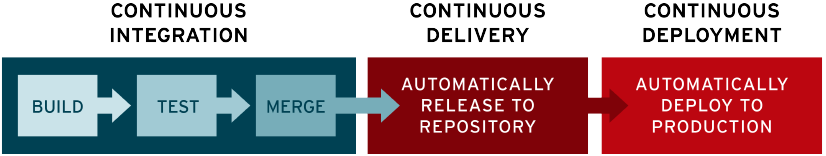
\includegraphics[width=0.75\textwidth]{ci-cd-flow-desktop}
    \caption{CI/CD tok}
\end{figure}

Moguće je da CI/CD obuhvati povezane prakse kontinualne integracije i kontinualnog dostavljanja, 
ili sve 3 povezane prakse kontinualne integracije, kontinualnog dostavljanja i kontinualnog 
raspoređivanja. Dodatnu komplikaciju stvara to što se kontinualna isporuka može nekada koristiti 
na način koji obuhvata procese kontinualnog raspoređivanja.

CI/CD je u stvari proces, često predstavljen kao tok, koji obuhvata uvođenje visokog stepena 
automatizacije i kontinualnog praćenja razvoja aplikacije.

Od slučaja do slučaja, na šta se termini konkretno odnose zavisi od toga koliko je automatizacije 
ugrađenou CI/CD tok. Mnoga preduzeća započinju dodavanjem CI, nakon čega uvode automatizaciju 
dostavljanja i raspoređivanja.

\subsection{Kontinualna integracija}
U razvoju modernih aplikacija, cilj je da više programera istovremeno radi na različitim delovima 
aplikacije. Međutim, ukoliko je organizacija postavljena tako da se spajanje koda sa svih grana 
vrši u jednom danu, takav posao može biti monoton, manuelan i dugotrajan. To se dešava u slučajevima 
kada programer vrši izmene na aplikaciji i na taj način povećava šansu za nastajanje konflikta sa 
izmenama koje istovremeno prave drugi programeri.

Kontinualna integracija (CI) pomaže programerima da spoje izmene na kodu na deljenu granu češće, 
čak i na dnevnom nivou. Nakon spajanja izmenjenih delova koda, izmene se validiraju tako što se 
automatski gradi aplikacija i pokreće se više nivoa automatskog testiranja. To znači da se testira 
sve, od klasa i funkcija do različitih modula koji su deo aplikacije. Ako automatski testovi pronađu 
konflikt između novog i postojećeg koda, CI nudi lako rešavanje konflikata.

\subsection{Kontinualna dostavljanje}
Nakon automatskog građenja aplikacije i testiranja u CI, kontinualno dostavljanje automatizuje 
puštanje prethodno validiranog koda na repozitorijum. Kako bismo imali efektivan proces kontinualne 
dostave, važno je da imamo već ugrađen CI u protoku. Cilj kontinualnog dostavljanja jeste postojanje 
baze koda koja je uvek spremna za raspoređivanje na produkciono okruženje.

U kontinualnom dostavljanju, svaka faza, počevši od spajanja izmenjenog koda do dostavljanja 
verzija spremnih za produkciju, podrazumeva automatsko testiranje i automatizaciju raspoređivanja 
koda. Na kraju tog procesa, operacioni tim je u mogućnosti da brzo i jednostavno rasporedi 
aplikaciju na produkciju.

\subsection{Kontinualno raspoređivanje}
Poslednja faza CI/CD protoka je kontinualno raspoređivanje. Kao dodatak kontinualnom dostavljanju, 
koji automatizuje isporuku verzija spremnih za produkciju, kontinualno raspoređivanje automatizuje 
puštanje aplikacije u produkciju. U velikoj meri se oslanja na dobro osmišljeno automatsko testiranje.

U praksi, kontinualno raspoređivanje znači da izmene na aplikaciji mogu biti na produkciji za samo 
nekoliko minuta (pod pretpostavkom da su automatski testovi uspešno završeni).

Sve povezane prakse CI/CD čine raspoređivanje aplikacije manje rizičnim, stoga je lakše pustiti 
promene u aplikaciji u delovima, pre nego odjednom.~\cite{CI_CD}

\subsection{GitHub Akcije}
Za verzionisanje koda se može koristiti GitHub. Pored verzionisanja, on pruža i alate za automatizaciju 
kontinualne integracije, isporue i raspoređivanja, kroz alat koji su nazvali \textit{Github Akcije} 
(eng. \textit{Github Actions}). 
GitHub Akcije su zasnovane na događajima, što znači da mogu da pokrenu niz komandi koje će se desiti 
posle navedenog događaja. Na primer, svaki put kada neko napravi \textit{zahtev za promenu} 
(eng. \textit{Pull Request}) nad repozitorijumu, može se automatski pokrenuti komanda koja pokreće 
testove. 

GitHub Akcije koriste YAML fajlove kako bi se definisale komponente toka rada. Ovi fajlovi 
se čuvaju u repozitorijumu, u folderu pod nazivom \mbox{\texttt{.github/workflows}}.

Komponente koje postoje u GitHub Akcijama su: 

\begin{itemize}
    \item Tok rada (eng. \textit{Workflow})
    \item Događaj (eng. \textit{Event})
    \item Posao (eng. \textit{Job})
    \item Korak (eng. \textit{Step})
    \item Akcija (eng. \textit{Action})
    \item Izvršilac (eng. \textit{Runner})
\end{itemize}

\begin{figure}[h]
    \centering
    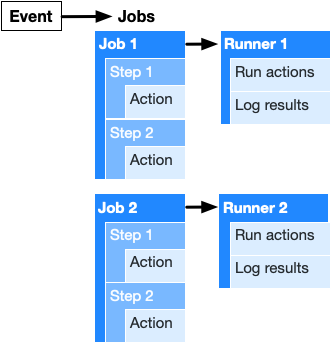
\includegraphics[width=0.5\textwidth]{overview-actions-design}
    \caption{Prikaz interakcija komponenata GitHub Akcija}
\end{figure}

\subsubsection{Tok rada}
Tok rada je automatizovana procedura koja se dodaje na repozitorijum. Tokovi radsa su sastavljeni 
od jednog ili više poslova i mogu se pokrenuti na određeni događaj ili biti zakazani u određeno vreme. 
Tok rada se može koristiti da se aplikacija izgradi, testira, spakuje, isporuči ili rasporedi na 
različita okruženja.

\subsubsection{Događaji}
Događaj je specifična aktivnost koja pokreće tok rada. Na primer, aktivnost može nastati kad neko napravi 
zahtev za promenu. Aktivnost ne mora da bude u okviru GitHub-a. Ona može doći preko poziva od strane 
nekog eksternog sistema.

\subsubsection{Posao}
Posao predstavlja skup koraka koji treba da se izvrše nad istim izvršiocem. Tok rada sa više poslova 
će pokrenuti ove poslove u paraleli. Naravno, tok rada se može podesiti tako da izvršava poslove 
sekvencijalno. Na primer, tok rada može imati dva sekvencijalna posla koji izgrađuju i testiraju kod, 
gde je posao za testiranje zavisan od toga da li kod uopšte može da se izgradi. Ako posao za izgradnju 
ne uspe, posao za testiranje se neće ni pokretati.

\subsubsection{Korak}
Korak predstavlja jednu zadatak koji može pokrenuti komandu unutar posla. Korak može biti ili akcija ili 
komandni skript. Svaki korak unutar posla se izvršava nad istim izvršiocem, što dozvoljava akcijama da 
dele podatke između sebe.

\subsubsection{Akcija}
Akcije predstavljaju samostalne komande koje se mogu kombinovati u korake kako bi sačinile jedan posao.
Akcije su najmanje portabilne jedinice građe toka rada. Korisnici mogu sami da naprave svoje akcije,
ili da koriste akcije koje su napravljene od strane GitHub zajednice. 

\subsubsection{Izvršilac}
Izvršilac je mašina nad kojom se GitHub Akcije izvršavaju. Izvršilac osluškuje pokrenute poslove,
pokreće jedan posao za drugim, i šalje izveštaje GitHub-u o napretku, logovima i rezultatima. Ove 
mašine mogu da budu bazirane na Linux, Windows i macOS operativnim sistemima, a svaki posao 
unutar toka rada se pokreće iz novog virtuelnog okruženja.~\cite{GitHubActions}
